\documentclass[a4paper, 12pt]{extarticle}
\usepackage[top=1in, bottom=1in, left=1in, right=1in]{geometry}
\usepackage{amsmath}
\usepackage{amssymb}
\usepackage{graphicx}
\usepackage{hyperref}
\usepackage{tcolorbox}
\usepackage{tikz}
\usepackage{enumitem}
\usepackage{fontspec}
\usetikzlibrary{calc,decorations,patterns,arrows,decorations.pathmorphing,positioning,shapes}
\definecolor{pltblue}{HTML}{1F77B4}
\definecolor{pltgreen}{HTML}{2CA02C}
\definecolor{pltred}{HTML}{D62728}
\definecolor{pltorange}{HTML}{FF7F0E}
\tikzset{every picture/.style={/utils/exec={\fontspec{Humor Sans}}}}
\setmainfont{Pretty Neat}

\makeatletter
\pgfset{
  /pgf/decoration/randomness/.initial=2,
  /pgf/decoration/wavelength/.initial=100
}
\pgfdeclaredecoration{sketch}{init}{
  \state{init}[width=0pt,next state=draw,persistent precomputation={
    \pgfmathsetmacro\pgf@lib@dec@sketch@t0
  }]{}
  \state{draw}[width=\pgfdecorationsegmentlength,
  auto corner on length=\pgfdecorationsegmentlength,
  persistent precomputation={
    \pgfmathsetmacro\pgf@lib@dec@sketch@t{mod(\pgf@lib@dec@sketch@t+pow(\pgfkeysvalueof{/pgf/decoration/randomness},rand),\pgfkeysvalueof{/pgf/decoration/wavelength})}
  }]{
    \pgfmathparse{sin(2*\pgf@lib@dec@sketch@t*pi/\pgfkeysvalueof{/pgf/decoration/wavelength} r)}
    \pgfpathlineto{\pgfqpoint{\pgfdecorationsegmentlength}{\pgfmathresult\pgfdecorationsegmentamplitude}}
  }
  \state{final}{}
}
\tikzset{xkcd/.style={decorate,decoration={sketch,segment length=0.5pt,amplitude=0.5pt}}}
\makeatother

\usepackage{etoolbox}
\AtBeginEnvironment{tabular}{\fontspec{Humor Sans}}

\setlength{\parindent}{0pt}
\setlength{\parskip}{0.5em}
\usepackage{fancyhdr}
\usepackage{geometry}
\usepackage{adjustbox}
\usepackage{titling}
\date{}

\title{Building Your Code Time Machine\\{\large A Discovery Exercise}}
\author{}
\date{}

\begin{document}

\maketitle

\section*{The Problem}

You're working on a data analysis project. You have a file called \texttt{analysis.py}. Over the course of a week, you make many changes. Sometimes you break things. Sometimes you fix them. Sometimes you want to remember what you did yesterday.

This exercise will help you discover a system for tracking your work.

\section{Part 1: Saving Your Work}

\subsection{Your First Day}

You start with this code in \texttt{analysis.py}:

\begin{tcolorbox}[colback=white, colframe=black]
\begin{verbatim}
def calculate_mean(data):
    total = sum(data)
    return total / len(data)
\end{verbatim}
\end{tcolorbox}

\begin{enumerate}
    \item You realize this code crashes when \texttt{data} is empty. You fix it:

\begin{tcolorbox}[colback=white, colframe=black]
\begin{verbatim}
def calculate_mean(data):
    if len(data) == 0:
        return 0
    total = sum(data)
    return total / len(data)
\end{verbatim}
\end{tcolorbox}

Write down exactly what changed (use \texttt{+} prefix for lines added, \texttt{-} prefix for lines removed):

\vspace{3cm}

    \item Later that day, you add a new function:

\begin{tcolorbox}[colback=white, colframe=black]
\begin{verbatim}
def calculate_mean(data):
    if len(data) == 0:
        return 0
    total = sum(data)
    return total / len(data)

def calculate_median(data):
    sorted_data = sorted(data)
    return sorted_data[len(sorted_data) // 2]
\end{verbatim}
\end{tcolorbox}

Write down what changed this time (use \texttt{+} prefix for lines added, \texttt{-} prefix for lines removed):

\vspace{3cm}

\end{enumerate}

\subsection{Designing a Tracking System}

\begin{enumerate}[resume]
    \item You want to remember what your code looked like at different points in time. For each snapshot you save, what three pieces of information would be essential to include? Consider: How will you know when this snapshot was created? How will you remember what changes you made? How will you know what the code looked like at this point?

\vspace{4cm}

    \item You decide to save snapshots in boxes. Here's what you have so far:

\begin{center}
\begin{tcolorbox}[colback=pltblue!10, colframe=pltblue, width=0.8\textwidth, title=Snapshot 1]
\textbf{When:} Monday 9:00 AM\\
\textbf{Message:} "Started project"\\
\textbf{Files:} analysis.py (original version)
\end{tcolorbox}
\end{center}

\end{enumerate}

\subsection{Choosing What to Save}

You spend all morning working. You now have:
\begin{itemize}
    \item \texttt{analysis.py} (finished, working perfectly)
    \item \texttt{test.py} (finished, working perfectly)
    \item \texttt{scratch.py} (messy experimental code, not ready)
    \item \texttt{temp\_output.txt} (temporary file, you don't need it)
\end{itemize}

\begin{enumerate}[resume]
    \item You want to create a snapshot. Should you include all four files?

    \vspace{2cm}

    \item You realize you need a way to choose which files go into a snapshot. Design a system with three areas:

    \begin{center}
    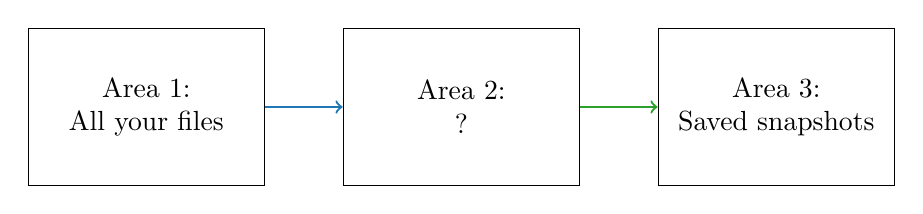
\begin{tikzpicture}[node distance=4cm]
        \node[draw, rectangle, minimum width=3cm, minimum height=2cm, align=center] (A) {Area 1:\\All your files};
        \node[draw, rectangle, minimum width=3cm, minimum height=2cm, align=center, right of=A] (B) {Area 2:\\?};
        \node[draw, rectangle, minimum width=3cm, minimum height=2cm, align=center, right of=B] (C) {Area 3:\\Saved snapshots};
        \draw[->, thick, pltblue] (A) -- (B);
        \draw[->, thick, pltgreen] (B) -- (C);
    \end{tikzpicture}
    \end{center}

    What should Area 2 be? What purpose does it serve? (Hint: Think about the problem you encountered with the four files earlier)

    \vspace{3cm}

    \item You have a file in Area 1 that you want to include in your next snapshot. What would you call the action of moving it to Area 2?

    \underline{\hspace{8cm}}

    You have files in Area 2 and you want to create a snapshot in Area 3 containing those files. What would you call this action?

    \underline{\hspace{8cm}}

    \vspace{1cm}

    \item Why is it useful to have Area 2 instead of going directly from Area 1 to Area 3?

    \vspace{3cm}

\end{enumerate}

\section{Part 2: Parallel Work}

\subsection{The Experiment Dilemma}

You want to try two completely different approaches to analyzing your data. You don't know which will work better. You want to try both without losing either one.

Your current snapshot history represents your stable, working code. This is the path that always works:

\begin{center}
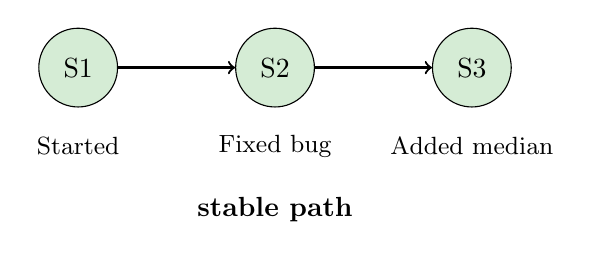
\begin{tikzpicture}[node distance=2.5cm]
    \node[draw, circle, fill=pltgreen!20, minimum size=1cm] (S1) {S1};
    \node[draw, circle, fill=pltgreen!20, minimum size=1cm, right of=S1] (S2) {S2};
    \node[draw, circle, fill=pltgreen!20, minimum size=1cm, right of=S2] (S3) {S3};
    \draw[->, thick] (S1) -- (S2);
    \draw[->, thick] (S2) -- (S3);
    \node[below of=S1, node distance=1cm] {\small Started};
    \node[below of=S2, node distance=1cm] {\small Fixed bug};
    \node[below of=S3, node distance=1cm] {\small Added median};
    \node[below of=S2, node distance=1.8cm] {\textbf{stable path}};
\end{tikzpicture}
\end{center}

\begin{enumerate}[resume]
    \item You want to try Method A and Method B starting from S3. Both will modify \texttt{analysis.py}. You want to keep the stable path stable and working. If you just keep making snapshots in a straight line on the stable path, what problem will you run into?

    \vspace{3cm}

    \item Starting from S3 on the stable path, you want to create snapshots for both Method A and Method B without losing either one or breaking the stable path. Draw what your snapshot history should look like. How can you arrange the snapshots so you can experiment with both methods while keeping the stable path stable?

    \vspace{5cm}

    \item You've created separate paths for experimentation while keeping the stable path stable. What would you call these experimental paths? Give them descriptive names based on what they're testing.

    \vspace{2cm}

\end{enumerate}

\subsection{Combining Work}

You and a colleague are both working on the project. You're working on different paths:

\begin{center}
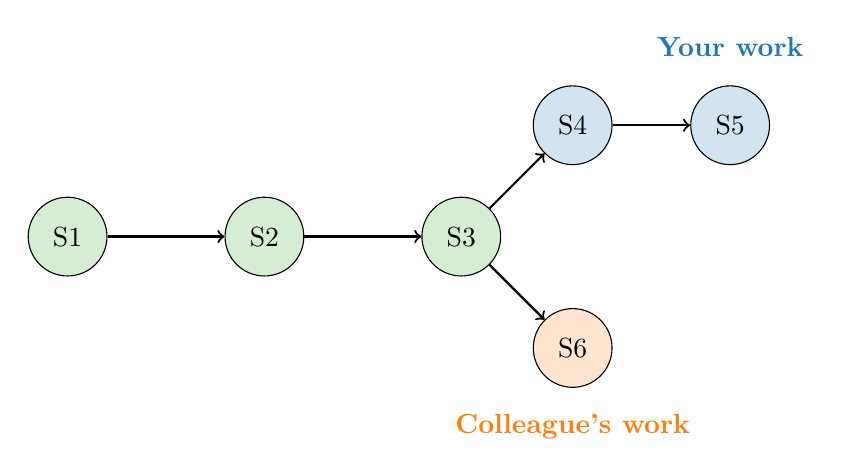
\begin{tikzpicture}[node distance=2.5cm]
    \node[draw, circle, fill=pltgreen!20, minimum size=1cm] (S1) {S1};
    \node[draw, circle, fill=pltgreen!20, minimum size=1cm, right of=S1] (S2) {S2};
    \node[draw, circle, fill=pltgreen!20, minimum size=1cm, right of=S2] (S3) {S3};
    \node[draw, circle, fill=pltblue!20, minimum size=1cm, above right of=S3, node distance=2cm] (S4) {S4};
    \node[draw, circle, fill=pltblue!20, minimum size=1cm, right of=S4, node distance=2cm] (S5) {S5};
    \node[draw, circle, fill=pltorange!20, minimum size=1cm, below right of=S3, node distance=2cm] (S6) {S6};

    \draw[->, thick] (S1) -- (S2);
    \draw[->, thick] (S2) -- (S3);
    \draw[->, thick] (S3) -- (S4);
    \draw[->, thick] (S4) -- (S5);
    \draw[->, thick] (S3) -- (S6);

    \node[above of=S5, node distance=1cm, color=pltblue] {\textbf{Your work}};
    \node[below of=S6, node distance=1cm, color=pltorange] {\textbf{Colleague's work}};
\end{tikzpicture}
\end{center}

In S4 and S5, you modified \texttt{analysis.py} to add feature X.\\
In S6, your colleague modified \texttt{README.md} to add documentation.

\begin{enumerate}[resume]
    \item You want to combine both sets of work into a single snapshot. Draw what the snapshot history should look like after combining:

    \vspace{5cm}

    \item Now imagine both you and your colleague modified the same line in \texttt{analysis.py}. You changed line 5 to:

    \texttt{result = data * 2}

    Your colleague changed line 5 to:

    \texttt{result = data * 3}

    When you try to combine the work, what problem occurs?

    \vspace{3cm}

\end{enumerate}

\clearpage

\section{Part 3: Collaboration}

\subsection{The Remote Backup Problem}

Your computer crashed last night. Luckily, your friend has been keeping backups of your snapshots on their server. But they only have up to S3. You had made it to S5 on your computer before the crash.

\begin{center}
\textbf{Your Computer (before crash):}
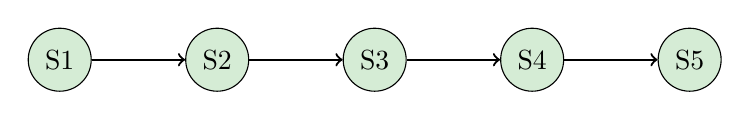
\begin{tikzpicture}[node distance=2cm]
    \node[draw, circle, fill=pltgreen!20, minimum size=0.8cm] (S1) {S1};
    \node[draw, circle, fill=pltgreen!20, minimum size=0.8cm, right of=S1] (S2) {S2};
    \node[draw, circle, fill=pltgreen!20, minimum size=0.8cm, right of=S2] (S3) {S3};
    \node[draw, circle, fill=pltgreen!20, minimum size=0.8cm, right of=S3] (S4) {S4};
    \node[draw, circle, fill=pltgreen!20, minimum size=0.8cm, right of=S4] (S5) {S5};
    \draw[->, thick] (S1) -- (S2);
    \draw[->, thick] (S2) -- (S3);
    \draw[->, thick] (S3) -- (S4);
    \draw[->, thick] (S4) -- (S5);
\end{tikzpicture}

\vspace{1cm}

\textbf{Backup Server:}
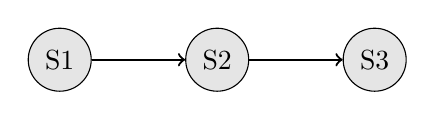
\begin{tikzpicture}[node distance=2cm]
    \node[draw, circle, fill=gray!20, minimum size=0.8cm] (S1) {S1};
    \node[draw, circle, fill=gray!20, minimum size=0.8cm, right of=S1] (S2) {S2};
    \node[draw, circle, fill=gray!20, minimum size=0.8cm, right of=S2] (S3) {S3};
    \draw[->, thick] (S1) -- (S2);
    \draw[->, thick] (S2) -- (S3);
\end{tikzpicture}
\end{center}

\begin{enumerate}[resume]
    \item The backup server has S1, S2, and S3. Your computer (before crashing) had S1 through S5. If you restore from the backup server, how much work will you need to redo? What specific changes from the scenario above would be lost?

    \vspace{2cm}

    \item What operation are you doing when you send snapshots to the backup server?

    \vspace{2cm}

    \item What operation are you doing when you retrieve snapshots from the backup server?

    \vspace{2cm}

\end{enumerate}

\subsection{Code Review}

You're working with a team. You've created a new feature on your path:

\begin{center}
\textbf{Backup Server:}
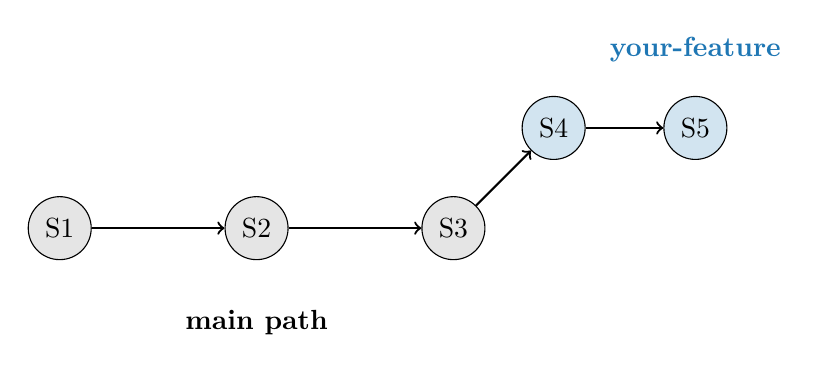
\begin{tikzpicture}[node distance=2.5cm]
    \node[draw, circle, fill=gray!20, minimum size=0.8cm] (S1) {S1};
    \node[draw, circle, fill=gray!20, minimum size=0.8cm, right of=S1] (S2) {S2};
    \node[draw, circle, fill=gray!20, minimum size=0.8cm, right of=S2] (S3) {S3};
    \node[draw, circle, fill=pltblue!20, minimum size=0.8cm, above right of=S3, node distance=1.8cm] (S4) {S4};
    \node[draw, circle, fill=pltblue!20, minimum size=0.8cm, right of=S4, node distance=1.8cm] (S5) {S5};

    \draw[->, thick] (S1) -- (S2);
    \draw[->, thick] (S2) -- (S3);
    \draw[->, thick] (S3) -- (S4);
    \draw[->, thick] (S4) -- (S5);

    \node[below of=S2, node distance=1.2cm] {\textbf{main path}};
    \node[above of=S5, node distance=1cm, color=pltblue] {\textbf{your-feature}};
\end{tikzpicture}
\end{center}

Your team has a rule: before combining work into the main path, someone else must review your code.

\begin{enumerate}[resume]
    \item Why might it be useful to have someone review your code before combining it?

    \vspace{3cm}

    \item Your teammate reviews S4 and S5. They leave comments on specific lines:

    \begin{tcolorbox}[colback=yellow!10, colframe=pltorange]
    \textbf{S5, analysis.py, line 12:}\\
    "This will crash if the input is negative. Can you add a check?"
    \end{tcolorbox}

    What are the specific steps you should take to address this feedback? Consider: Do you need to create a new snapshot? Should the new work go on the same path or a different one? How will your teammate know you've addressed their concern?

    \vspace{3cm}

\end{enumerate}

\section{Part 4: The Complete System}

\subsection{The Complete System}

You've now designed a complete system for tracking code changes and collaborating with others.

\begin{enumerate}[resume]
    \item Summarize your system by describing: (1) How you save and track changes over time, (2) How you choose what to include in each save, (3) How you work on multiple versions simultaneously, (4) How you combine different people's work, and (5) How you synchronize work across computers.

    \vspace{8cm}

\end{enumerate}

\subsection{The Real Names}

The system you just designed is called \textbf{Git}. Here are the real names for the concepts you discovered:

\begin{tcolorbox}[colback=pltblue!10, colframe=pltblue]
\begin{itemize}
    \item \textbf{Snapshot} = Commit
    \item \textbf{Area 2 (choosing what to save)} = Staging Area
    \item \textbf{Parallel paths} = Branches
    \item \textbf{Combining work} = Merge
    \item \textbf{Backup server} = Remote Repository (e.g., GitHub)
    \item \textbf{Sending to server} = Push
    \item \textbf{Getting from server} = Pull
    \item \textbf{Code review request} = Pull Request
    \item \textbf{Change notation} = Diff
\end{itemize}
\end{tcolorbox}

\begin{enumerate}[resume]
    \item Now that you know the real names, write a short description of what Git is and why it's useful:

    \vspace{5cm}

\end{enumerate}

\end{document}
